\documentclass[12pt,a4paper,titlepage]{article}
\usepackage[utf8]{inputenc}
\usepackage[spanish]{babel}
\usepackage{listings}
\usepackage{color}
\usepackage{graphicx}
\usepackage{float}

\definecolor{mygreen}{rgb}{0,0.6,0}
\definecolor{mygray}{rgb}{0.5,0.5,0.5}
\definecolor{mymauve}{rgb}{0.58,0,0.82}


%opening
\title{Contribuyendo a Python}
\author{Emmanuel Arias}

\begin{document}
\lstset{
	language=Python,
    showspaces=false,
	numbers=left,
	keywordstyle=\color{blue},
	numbersep=5pt,
	numberstyle=\color{mygray},
	rulecolor=\color{black},
	stringstyle=\color{mymauve}}

\maketitle

\tableofcontents

\newpage

\section{Introducción}
La mayoría de los proyectos FOS\footnote{Free and Open Source} son mantenidos y llevados
a cabo por desarrolladores en su tiempo libre. Un bajo porcentaje
de ellos son pagados. Por lo tanto, es necesario que mientras más
personas se involucren en el software libre, se tendrá mejores
softwares, con menos bugs, y que brinden una mejor experiencia.

Cabe aclarar que el software libre está ganando terreno frente al
privativo. Solo para mencionar algunos ejemplos, el kernel linux
lidera el mercado de servidores, cómo así también el de smartphones
con Android. Apache y Nginx en servidores web. Scikit-learn, Python 
para el lado del Machine Learning. Pero, dónde el software privativo
(Windows) sigue teniendo la supremacía es en las computadoras 
de escritorio. 

Hoy en día introducirse a contribuir en el software libre no es
tan complicado, gracias a la gran comunidad que se forman alrededor
de los proyectos FOS. En este trabajo, se pone énfasis en el
proyecto Python y su comunidad. 

\section{Python}
Python es un lenguaje de programación interpretado y de propósito
general, tipado dinámico, multiplataforma y de código abierto.
El lenguaje fue creado por Guido van Rossum, y en 1991 tuvo
su primera release. Python tienen como filosofía que el código
escrito sea legible, con una sintaxis sencilla. Además, nace
para ser un lenguaje fácil de aprender y de rápida implementación. Es
por estos motivos que Python se ha vuelto muy popular.

En base a lo mencionado anteriormente Tim Peters, un ingeniero de 
software y uno de los mayores contribuidores del lenguaje y de la
primera implementación del interprete de Python, ha escrito
el Zen de Python\footnote{\textit{python -c "import this"}}, el cual dice:
\\

\itshape
\textbf{The Zen of Python, by Tim Peters}
\\
Beautiful is better than ugly.
Explicit is better than implicit.\\
Simple is better than complex.\\
Complex is better than complicated.\\
Flat is better than nested.\\
Sparse is better than dense.\\
Readability counts.\\
Special cases aren't special enough to break the rules.\\
Although practicality beats purity.\\
Errors should never pass silently.\\
Unless explicitly silenced.\\
In the face of ambiguity, refuse the temptation to guess.\\
There should be one-- and preferably only one --obvious way to do it.\\
Although that way may not be obvious at first unless you're Dutch.\\
Now is better than never.\\
Although never is often better than *right* now.\\
If the implementation is hard to explain, it's a bad idea.\\
If the implementation is easy to explain, it may be a good idea.\\
Namespaces are one honking great idea -- let's do more of those!\\ \normalfont

Python es un lenguaje de programación multi-paradigma, por lo tanto
soporta programación orientada a objetos, programación estructurada,
programación funcional, etc.

Como se mencionó anteriormente, Python fue creado para ser ``de fácil
lectura". A diferencia de otros lenguajes no usa llaves para separar
bloques de códigos, sino que se usa la indentación, por 
recomendación 4 espacios en blanco\footnote{pep8: https://www.python.org/dev/peps/pep-0008/}),
en vez de la tabulación (\textit{\textbackslash t}) esto ayuda a identificar
rápidamente los diferentes bloques de código. Por ejemplo:

\begin{lstlisting}
def print_name_10_times(name):
    for i in range(10):
        print(name)
    print('Bye Bye')
\end{lstlisting}

Python además de poder ser ejecutado por medio de un archivo ``.py'', el
intérprete permite la ejecución a través de un modo interactivo. Con esto se puede
introducir las instrucciones y evaluar directamente su resultado. 

\subsection{¿Python un lenguaje nuevo?}
Guido van Rossum comenzó el desarrollo de Python en diciembre de
1989\footnote{http://python-history.blogspot.com/2009/01/brief-timeline-of-python.html}.
Empezó como un hobbie en las vacaciones de Navidad. El 20 de febrero de 1991 tiene su
primera release: 0.9.0 (en alt.sources). El 26 de enero de 1994 se lanza la versión 1.0.0.
En octubre del 2000 se lanza Python 2.0 y el 3 de diciembre de 2008 se lanza la versión
3.0.

Actualmente, se puede observar que existe un ``boom'' en el uso de Python, esto se debe
a la popularización tanto de frameworks web como Django o Flask, como así
también del uso de Machine Learning en la industria y educación. Sumado al
desarrollo de una gran cantidad de módulos (bibliotecas) que facilitan el desarrollo.

Pero esto no significa que sea un lenguaje nuevo. Por ejemplo, JavaScript tuvo su primera
release el 4 de diciembre de 1995 y Java tuvo su primera release el 23 de mayo de 1995.
Por otro lado Ruby tuvo su primera aparición en 1995. Esto significa que Python es más 
antiguo que los lenguajes mencionados anteriormente.

\section{PSF y PyAr}
Python no es solo un lenguaje de programación. Existe una gran comunidad detrás de Python,
que impulsa el continuo crecimiento del lenguaje y su comunidad. La Python Software
Foundation tiene como misión promover, proteger y avanzar el lenguaje de programación Python, 
como así también dar soporte al crecimiento de una comunidad diversa e internacional de 
programadores Python\footnote{https://www.python.org/psf/mission/}.

En Argentina existe Python Argentina (PyAr)\footnote{https://www.python.org.ar/}. PyAr al
igual que PSF busca promover el uso de Python e intercambiar información. Es la encargada
de realizar las conferencia de Python en Argentina, llamadas PyConAr, dónde se llevan a cabo
divulgaciones sobre el lenguaje. Además, organiza las denominadas PyCamp, que son campamentos
dónde los participantes pasan algunos días, comúnmente un fin de semana largo, realizando
contribuciones a proyectos tanto argentinos como internacionales. PyAr realiza este tipo
de actividades y muchas más, con el objetivo de hacer crecer la comunidad Python en Argentina.

\section{¿Puedo contribuir a Python?}
Al igual que cualquier proyecto de código abierto, la comunidad incentiva las contribuciones.
La gran mayoría de los proyectos FOS son gratuitos, y son proyectos mantenidos mayormente,
por personas en su tiempo libre. Esto significa que los desarrollos pueden llegar a ser 
muy lentos en algunos casos, por lo tanto, mientras más ayuda se reciba es mejor. No se
necesita ser un programador Senior para comenzar a contribuir, siempre hay espacio para todos.
Tampoco es necesario ser desarrollador, hay mucha ayuda ``no técnica'' que se necesita,
documentación, divulgador, o simplemente usar el software y reportar los bugs que se encuentran.

A continuación se describen algunos proyectos que son mantenidos por la comunidad Python.

\subsection{CPython}
CPython es el principal interprete de Python, escrito en C. Si bien, podríamos mencionar
que este interprete es el ``oficial'', existen varios otros interpretes escritos en
diferentes lenguajes por ejemplo: Jython, que corre en Java Virtual Machine; IronPython, que 
corre en .NET; MicroPython que es un Python que permite ser ejecutado en microcontroladores;
PyPy, el cual es un interprete escrito en Python.

Un buen lugar para comenzar a contribuir en CPython (se podría decir que obligatorio) es 
el Python Developer's Guide\footnote{https://devguide.python.org/}. Esta guía, que es
mantenida por la misma comunidad y brinda una breve introducción de cómo funciona CPython,
y de cómo es el proceso para contribuir en el lenguaje Python.

CPython se encuentra alojado en GitHub\footnote{https://github.com/python/cpython}.
\\
\begin{figure}[H]
	\centering
	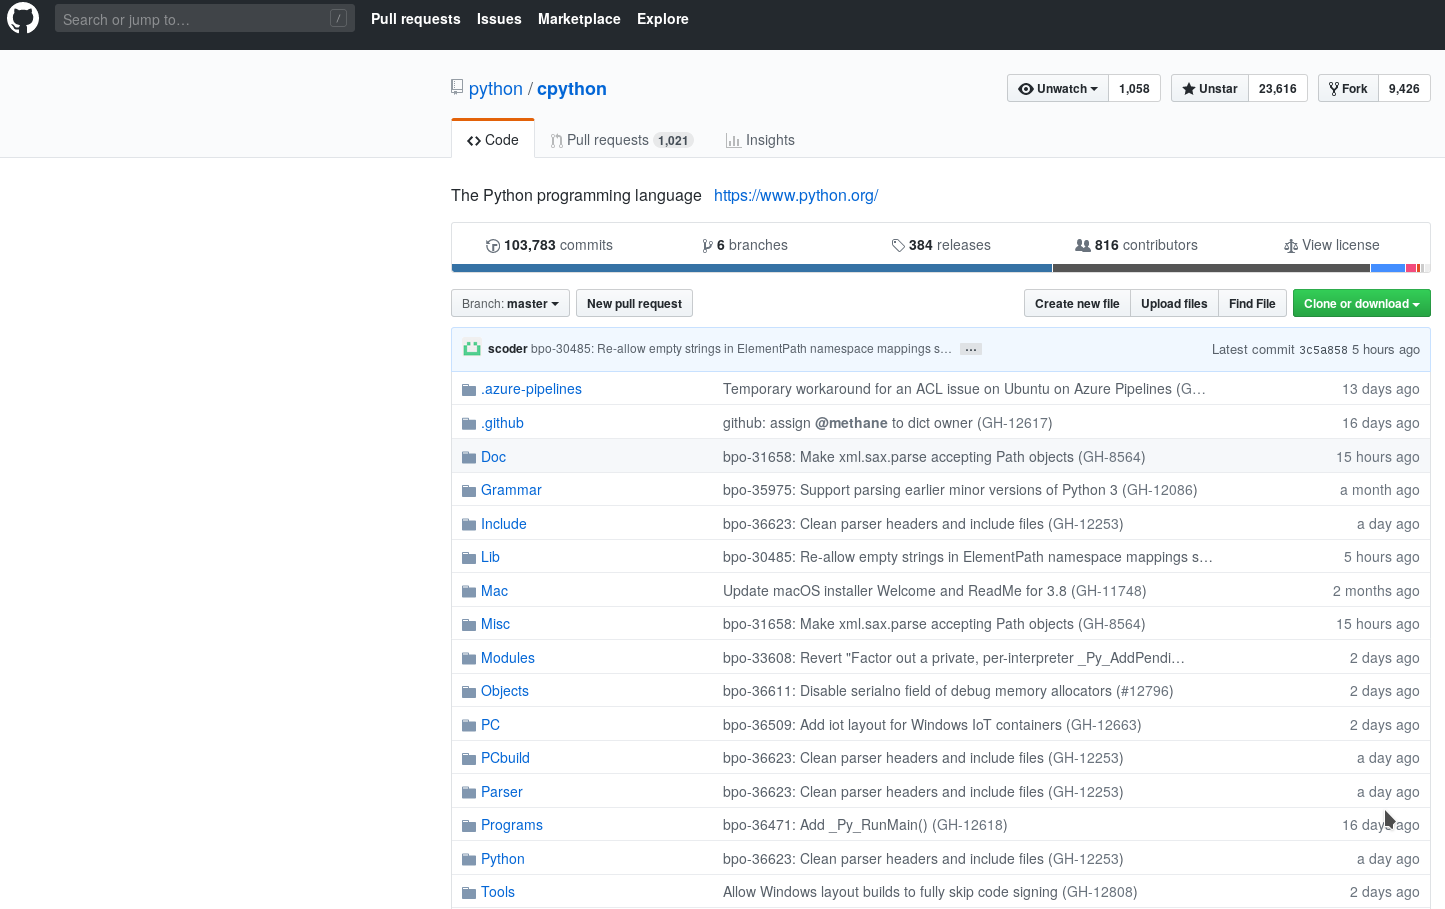
\includegraphics[width=0.7\linewidth]{github}
	\caption[CPython on Github]{CPython on Github}
	\label{fig:github}
\end{figure}

Para poder acceder al código, para luego poder crear patches (Pull Request en GitHub)
es necesario contar con un usuario y realizar un fork. 

\begin{figure}[H]
	\centering
	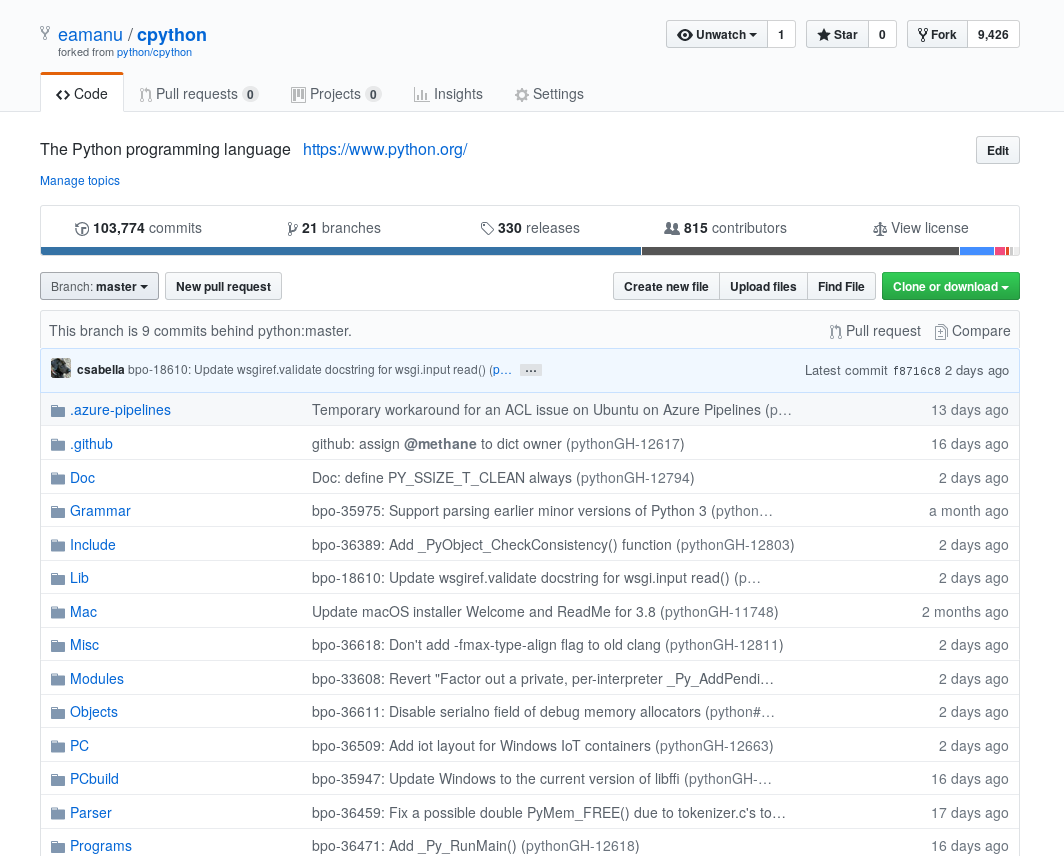
\includegraphics[width=0.7\linewidth]{fork}
	\caption[Fork CPython]{Fork CPython}
	\label{fig:fork}
\end{figure}

Luego se debe realizar un clonado del proyecto:

\begin{lstlisting}[language=Bash]
git clone git@github.com:eamanu/cpython.git
\end{lstlisting}

Una vez realizado el clonado del proyecto, ya podremos empezar a estudiar el código,
resolver bugs y agregar nuevas features.

Los bugs de Python son registrados en https://bugs.python.org. Este es un bugs tracker
dónde usuarios registrados pueden levantar bugs (o supuestos bugs). Los bugs son 
clasificados, ya sea que es un bugs para el interprete propiamente dicho, las librerías
estándar, compilación, documentación, etc. Aquellos bugs que necesiten ser debatidos, 
debido a su complejidad o a que representan cambios importantes en el funcionamiento o 
implementación del intérprete o lenguaje son dirigidos a la lista de mail 
\textit{python-dev}\footnote{https://mail.python.org/pipermail/python-dev/} o en 
http://discuss.python.org/.

\begin{figure}[H]
	\centering
	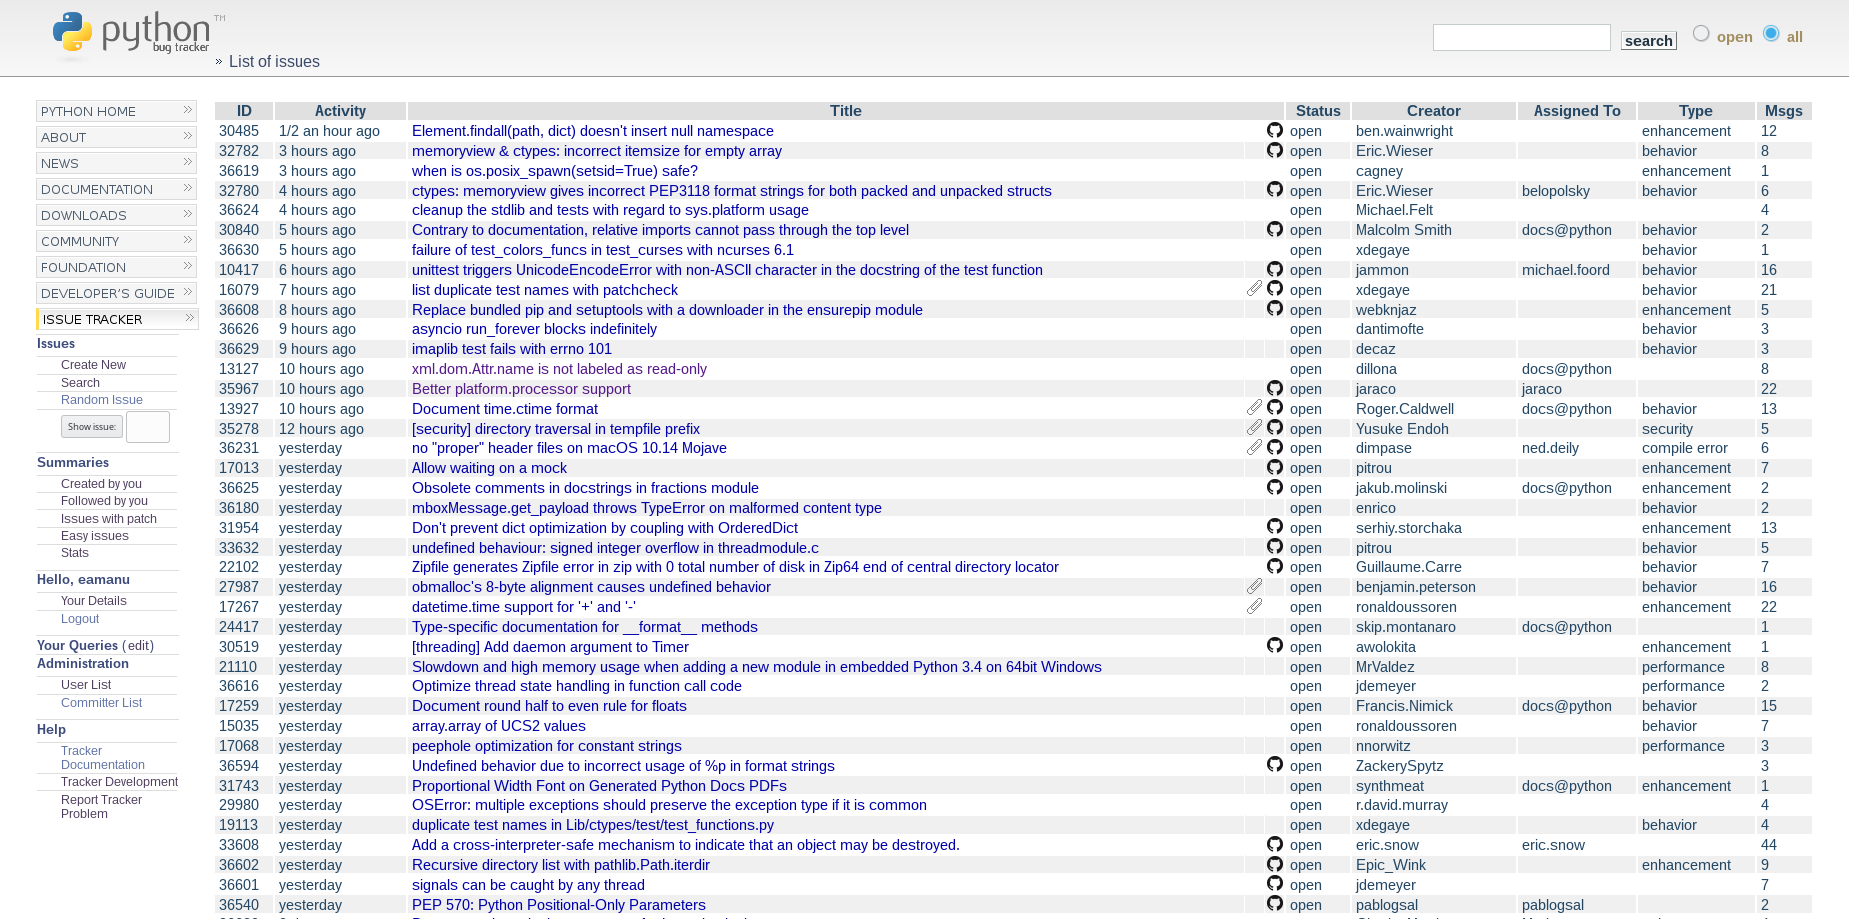
\includegraphics[width=0.7\linewidth]{bpo}
	\caption{bugs.python.org}
	\label{fig:bpo}
\end{figure}

También existe una sección de bugs en \textbf{bpo} que concentra \textit{easy issues}
que está pensado para aquellos que quieran realizar sus primeras contribuciones.

Se puede acceder a ayuda por parte de Core Devs o contribuidores experimentados vía
IRC en el canal \textit{\#python-dev} o en \textit{https://python.zulipchat.com}

\subsection{Otros proyectos}

Existen además, muchos otros proyectos que son soportados por la comunidad de Python.
Entre ellos podemos mencionar la misma página web de python \textbf{pythondotorg},
las python enhancement proposal \textbf{peps}, la guía de
desarrolladores \textbf{devguide}.

\begin{figure}[H]
	\centering
	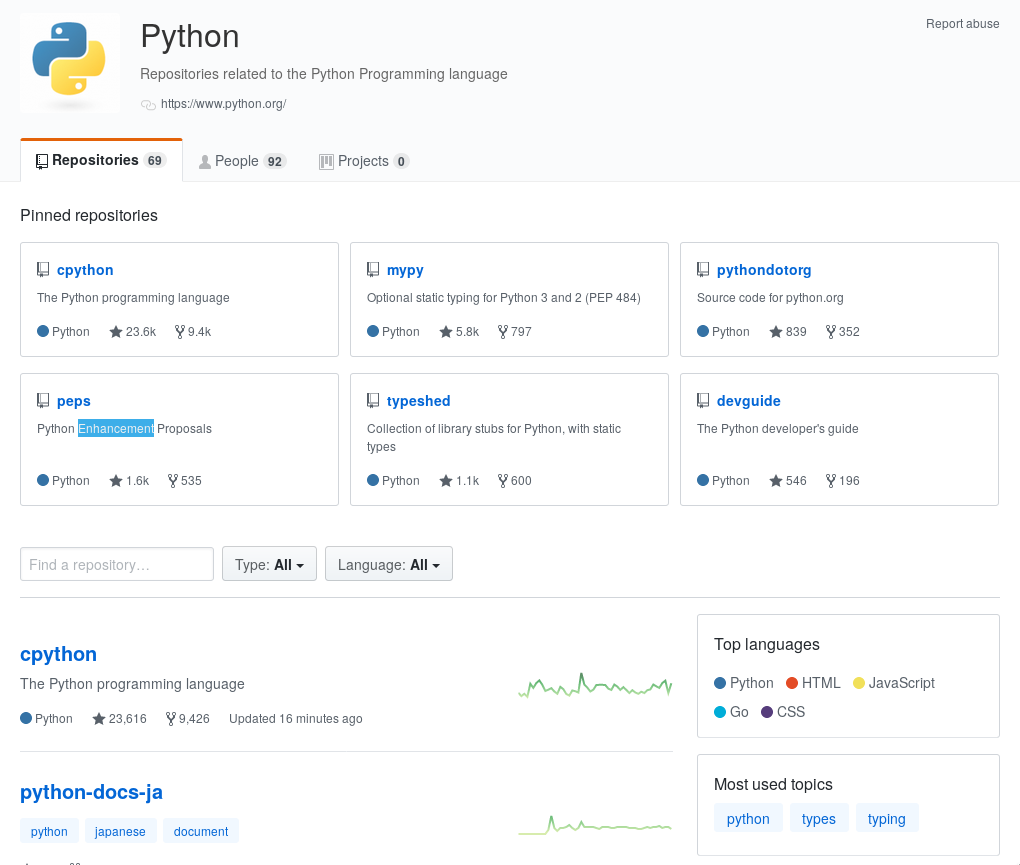
\includegraphics[width=0.7\linewidth]{repositories}
	\caption{Repositorios de Python}
	\label{fig:repositories}
\end{figure}

Python Argentina también tiene proyectos, se puede mencionar por ejemplo aquellos 
que buscan tener participación en el Google Summer of Code 2019:
\begin{itemize}
	\item CDPedia: Wikipedia offline.
	\item PyZombies: MOOC Español, tutoriales de Python.
	\item PyArWeb: Sitio oficial de Python Argentina.
	\item OpenLex: Manejo de estudios jurídicos y oficinas judiciales.
	\item PyAFIP WS: Factura electrónica y aplicativos.
	\item fades: easy virtualenv wrapper.
\end{itemize}
\section{Conclusión}
Python, al igual que muchos proyectos open source cuentan con una gran comunidad,
tanto de desarrolladores, como divulgadores y usuarios que contribuyen para que 
el mismo siga creciendo y desarrollándose. El objetivo de este trabajo, es mostrar
una pequeña parte de lo que es Python, y una más pequeña parte de lo que es la 
comunidad de open source.

\end{document}
